%mark = star, diamond, square, otimes
%\documentclass{article}
%\usepackage{pgfplots}
%\usepackage[justification=centering]{caption}
%\pgfplotsset{compat=newest}
%\begin{document}
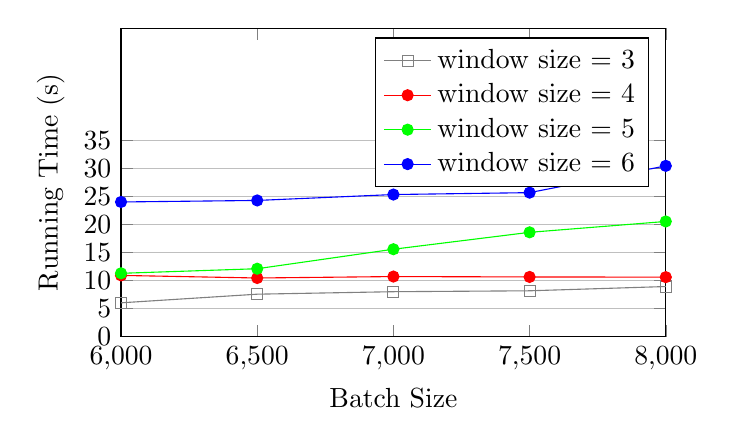
\begin{tikzpicture}
\begin{axis}[
    width=8.5cm,
    height=5.5cm,
    xlabel={Batch Size},
    ylabel={Running Time (s)},
    xmin=6000, xmax=8000,
    ymin=0, ymax=55,
    xtick={6000,6500,7000,7500,8000},
    ytick={0,5,10,15,20,25,30,35},
    legend pos=north east,
    ymajorgrids=true,
    grid style={line width=.2pt,draw=gray!50},
]
 
\addplot[
    solid,color=gray, every mark/.append style={solid, fill=gray}, mark=square
    ]
    coordinates {
		(6000,6.048)
		(6500,7.587 )
		(7000,8.030 )
		(7500,8.192 )
		(8000,8.951 )
	};
    \addlegendentry{window size $=$ 3}

	\addplot[
    solid,color=red, every mark/.append style={solid, fill=red}, mark=*
    ]
    coordinates {
		(6000,10.935)
		(6500,10.473)
		(7000,10.729)
		(7500,10.662)
		(8000,10.625)

};
    \addlegendentry{window size $=$ 4}
	

\addplot[
    solid,color=green, every mark/.append style={solid, fill=green}, mark=*
    ]
    coordinates {
		(6000,11.308)
		(6500,12.126)
		(7000,15.602)
		(7500,18.613)
		(8000,20.552)

};
    \addlegendentry{window size $=$ 5}
	
	
\addplot[
    solid,color=blue, every mark/.append style={solid, fill=blue}, mark=*
    ]
    coordinates {
		(6000,24.026)
		(6500,24.299)
		(7000,25.351)
		(7500,25.690)
		(8000,30.460)

};
    \addlegendentry{window size $=$ 6}
\end{axis}
\end{tikzpicture}
%\end{document}